\FormatSizeA{1}{%
\section {Пример добавления рисунка во весь формат на лист большого размера, и соответствующей подрисуночной подписи} \label{app:SCH_pult}

\begin{figure}[H]%
\unitlength=1mm%
 \begin{picture}(0, 500)(25.2, -540)% Волшебные чиселки. Их лучше не трогать, а то картинки расползутся и подпись к рисунку уползёт
 %   \begin{picture}(600,480)(25,549.5)% Волшебные чиселки. Их лучше не трогать, а то картинки расползутся и подпись к рисунку уползёт
    \put(0,0){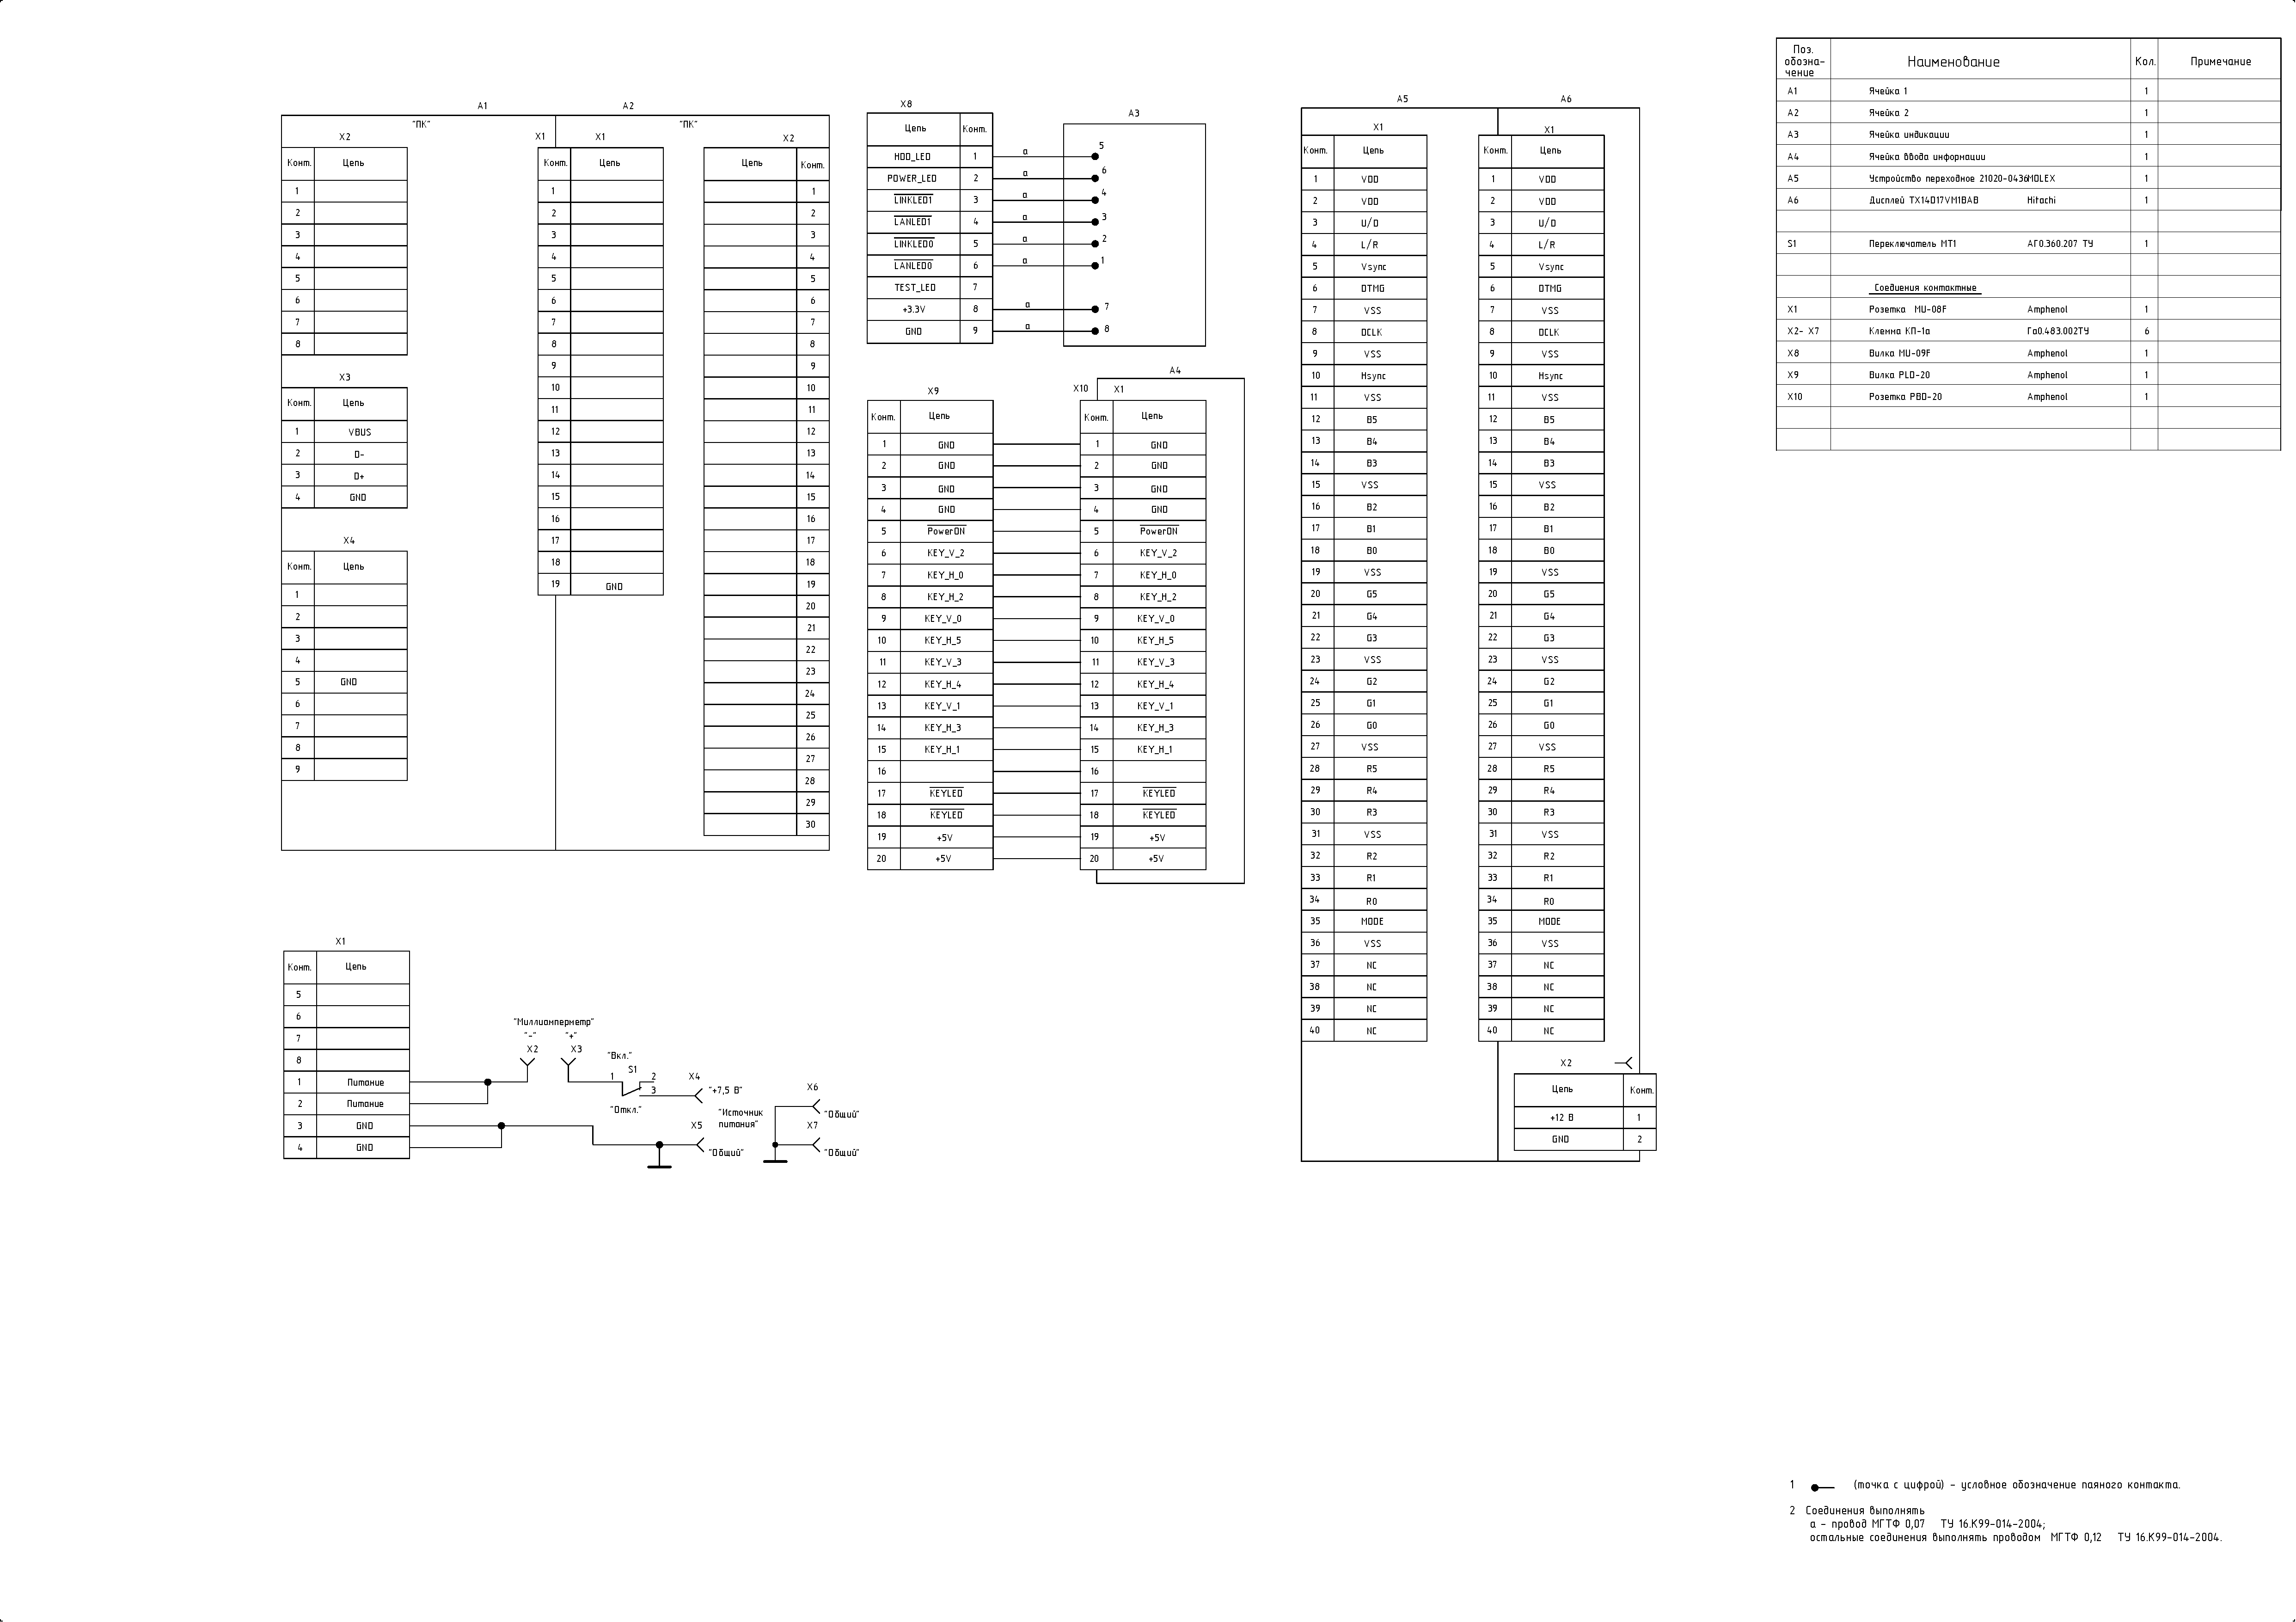
\includegraphics[scale=1.0,  angle=270]{./about/A1_example}}% Волшебные чиселки. Их лучше не трогать, а то картинки расползутся и подпись к рисунку уползёт
  \end{picture}%

  \captionsetup{width=170mm,
                margin={250mm,-250mm}
                }%
  \caption{Схема электрическая принципиальная пульта для программирования} \label{a:p:pult_main}
\end{figure}%

}%






\FormatSizeA{2}{%

\begin{figure}[H]%
\unitlength=1mm%
%  \begin{picture}(300,350)(25,54.7)% Волшебные чиселки. Их лучше не трогать, а то картинки расползутся и подпись к рисунку уползёт
  \begin{picture}(0, 350)(25.2, -365)% Волшебные чиселки. Их лучше не трогать, а то картинки расползутся и подпись к рисунку уползёт
    \put(0,0){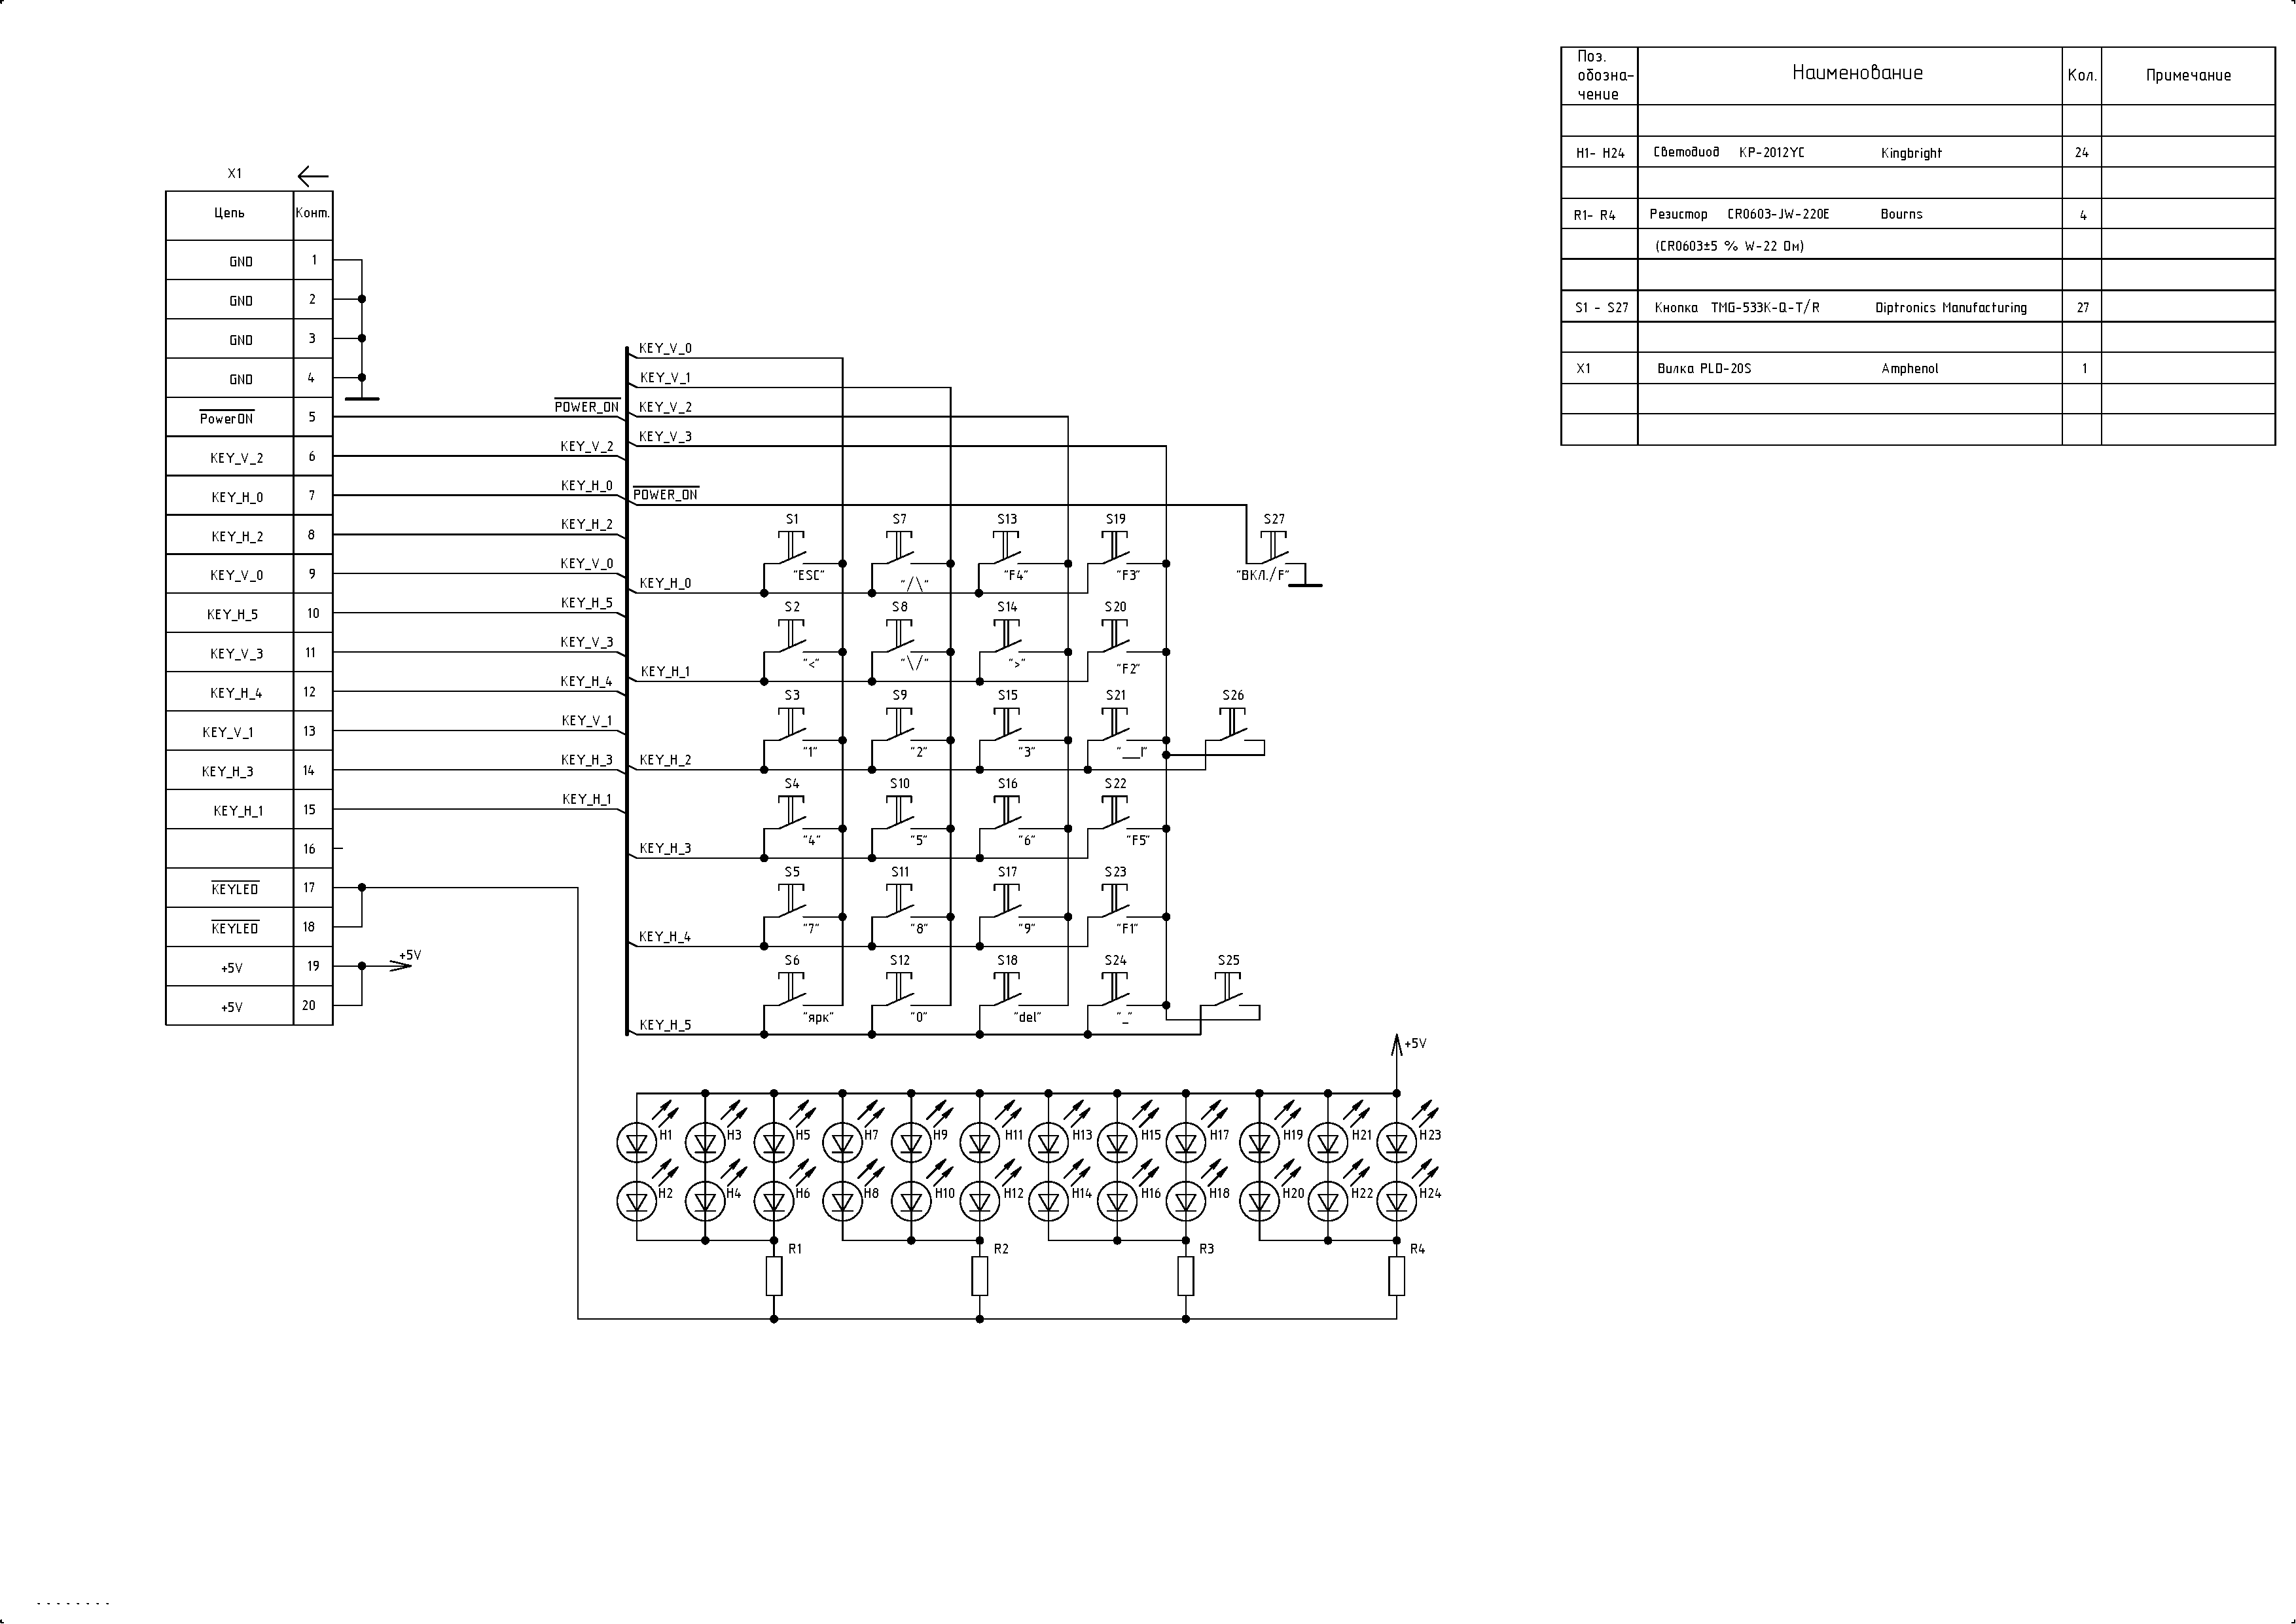
\includegraphics[ scale=1, angle=-90]{./about/A2_example}}% Волшебные чиселки. Их лучше не трогать, а то картинки расползутся и подпись к рисунку уползёт
  \end{picture}%

  \captionsetup{width=170mm,
                margin={150mm,-150mm}
                }%
  \caption{Схема электрическая принципиальная ячейки ввода информации} \label{a:p:pult_main_part1}
\end{figure}%

}%



\FormatSizeA{4}{%

\begin{figure}[H]%
\unitlength=1mm%
  \begin{picture}(0,235)(26,50)% Волшебные чиселки. Их лучше не трогать, а то картинки расползутся и подпись к рисунку уползёт
    \put(0,0){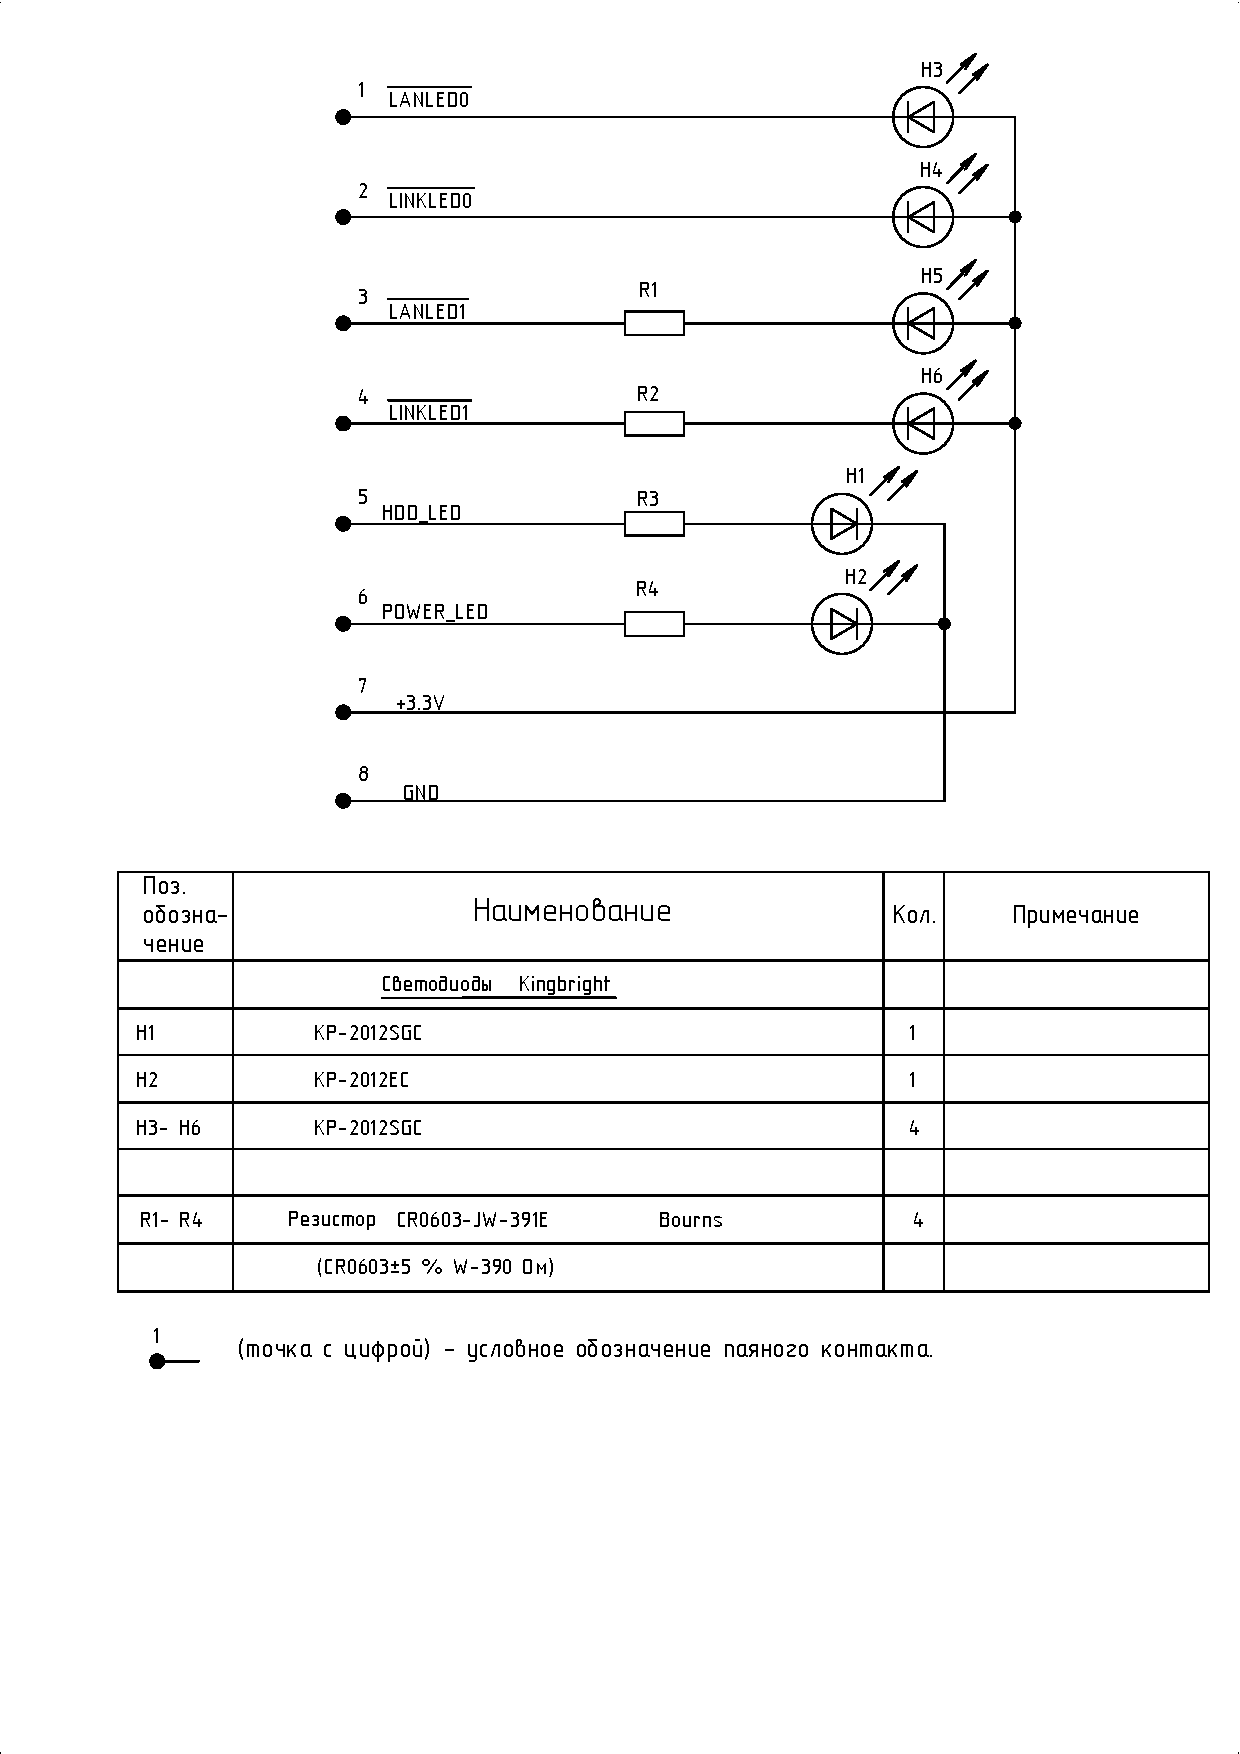
\includegraphics[scale = 1.004]{./about/A4_v_example}}% Волшебные чиселки. Их лучше не трогать, а то картинки расползутся и подпись к рисунку уползёт
  \end{picture}%
  \caption{Схема электрическая принципиальная ячейки индикации} \label{a:p:pult_main_part2}
\end{figure}%

}%


\FormatSizeA{3}{%
%\section {Схема электрическая подключения устройства} \label{app:SCH_all_units}
\
\

\begin{figure}[H]%
\unitlength=1mm%
  \begin{picture}(0,225)(25.2 ,-250)% Волшебные чиселки. Их лучше не трогать, а то картинки расползутся и подпись к рисунку уползёт
    \put(0,0){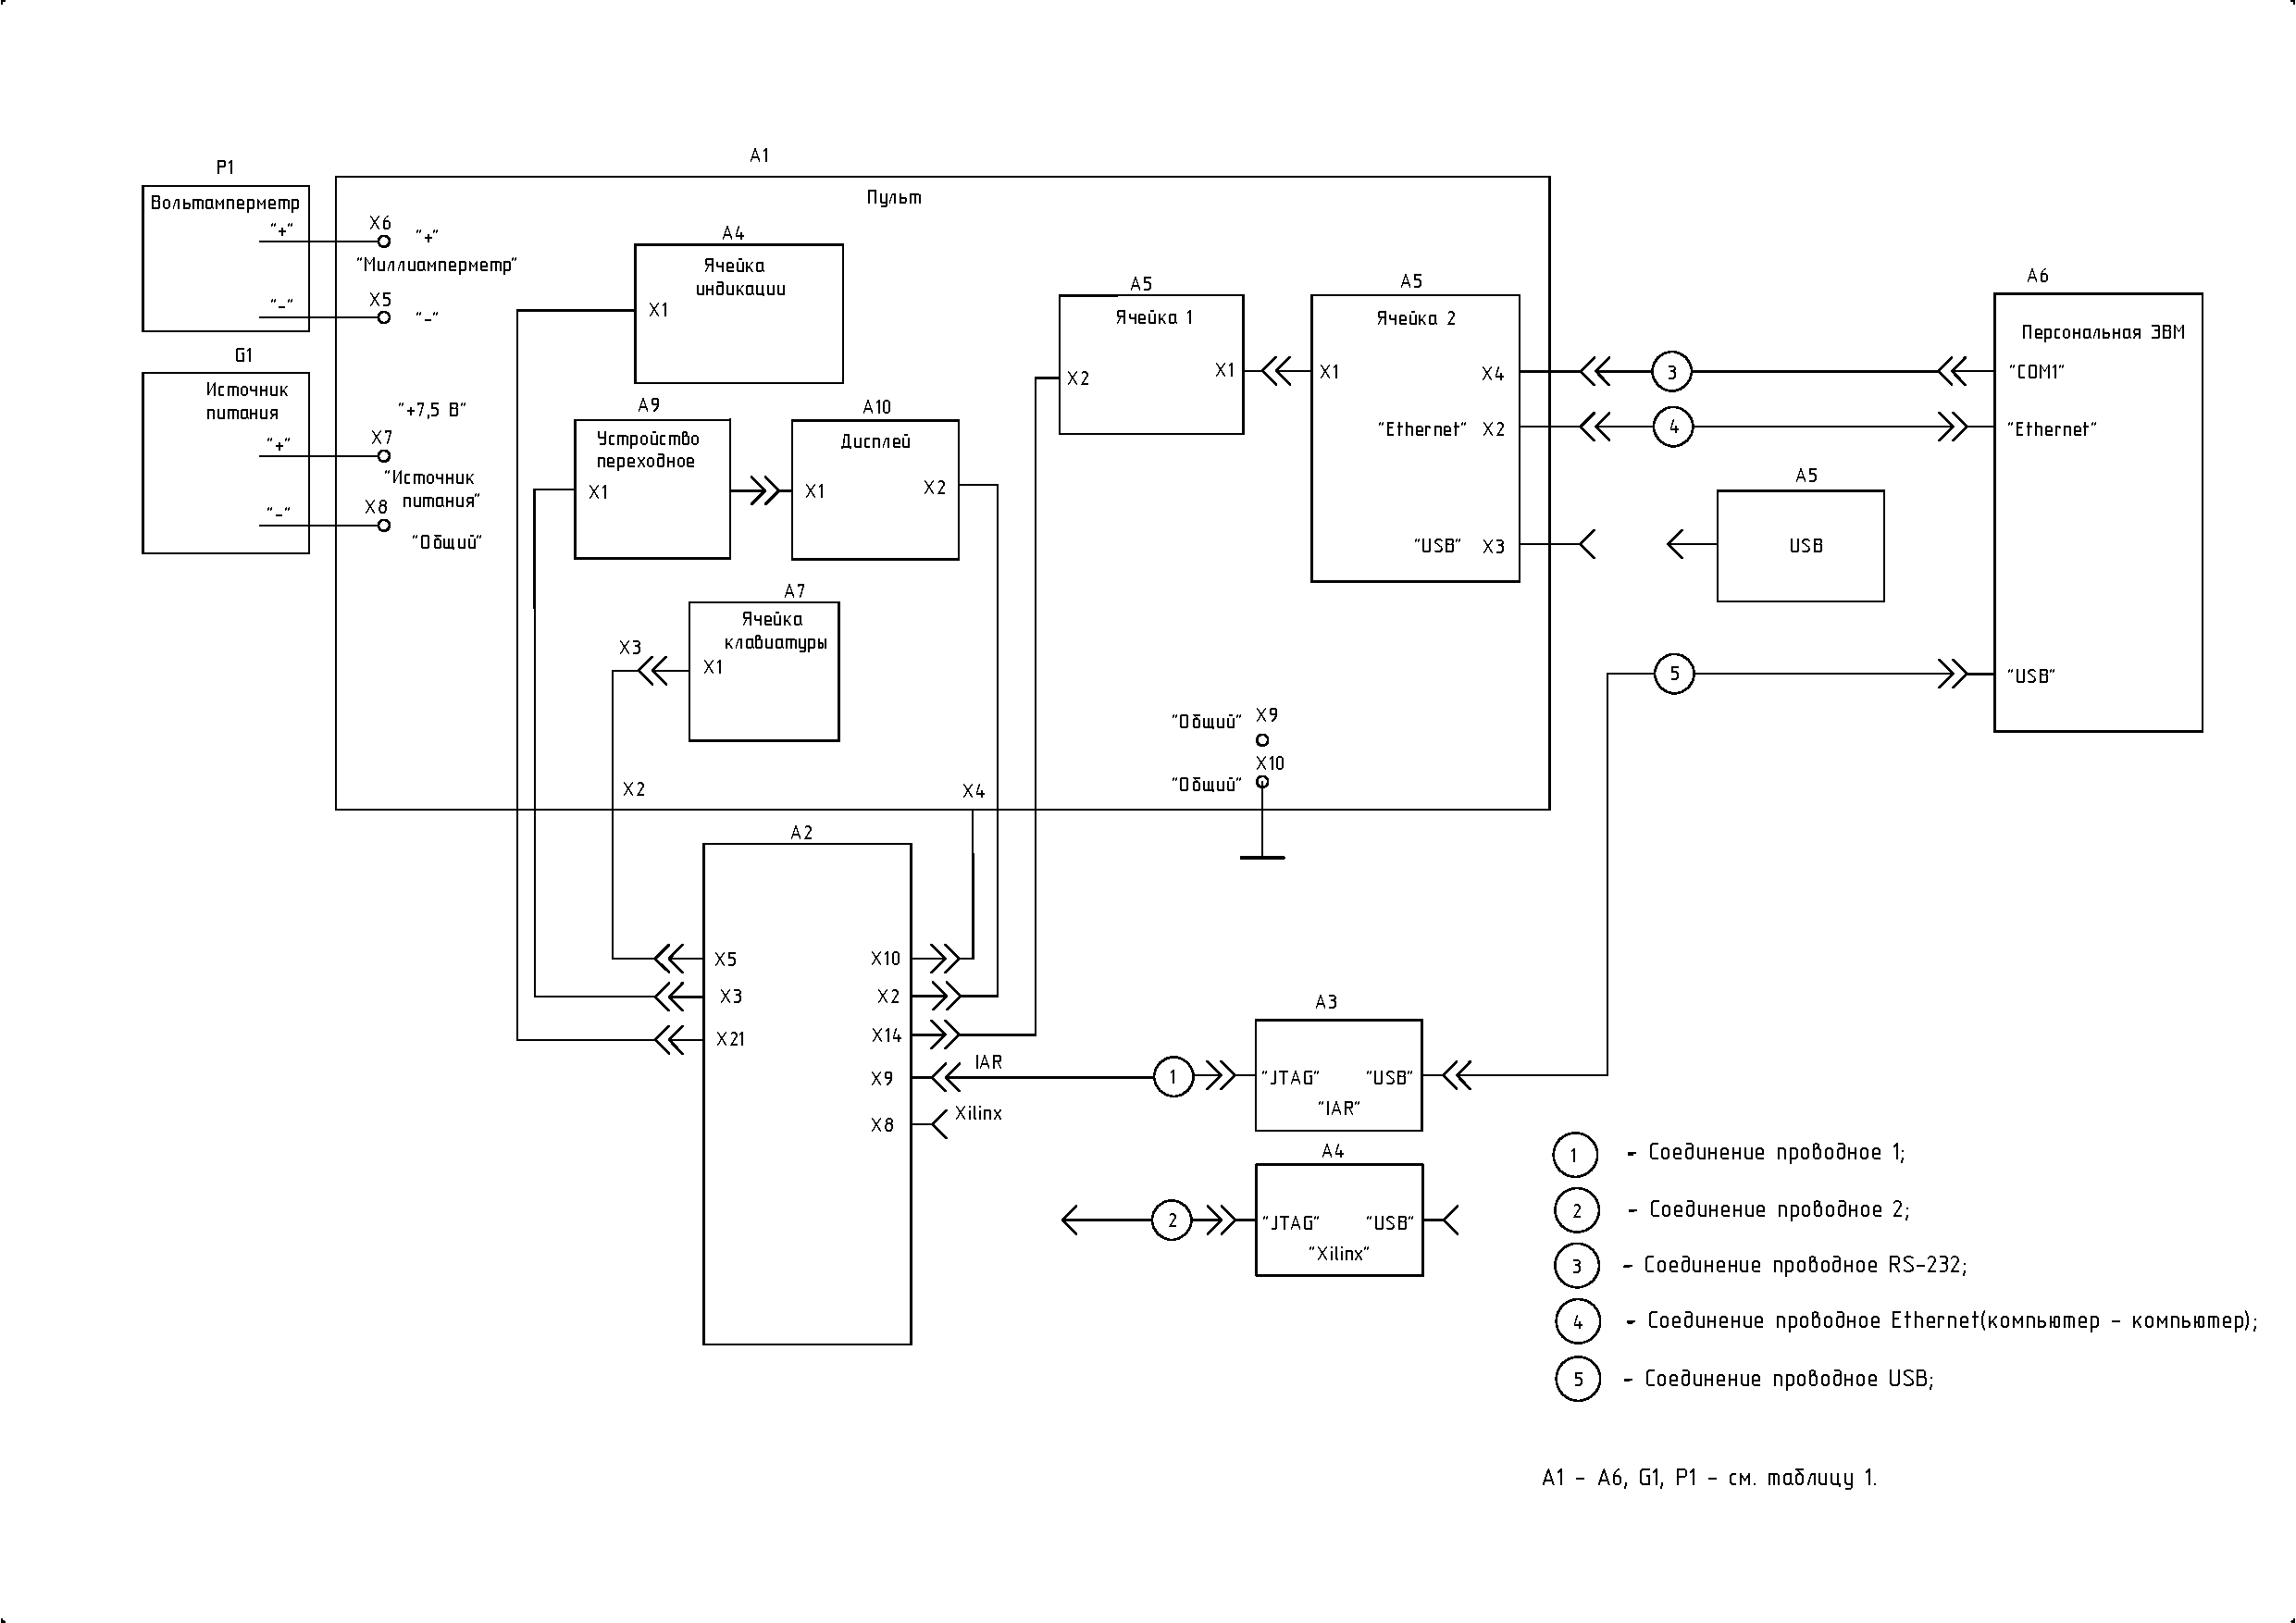
\includegraphics[ scale=1, angle=-90]{./about/A3_example}}% Волшебные чиселки. Их лучше не трогать, а то картинки расползутся и подпись к рисунку уползёт
  \end{picture}%

  \captionsetup{width=170mm,
                margin={-50mm,-150mm}
                }%
  \caption{Схема электрическая подключения устройства} \label{a:p:SCH_all_units}
\end{figure}%

}%













\FormatSizeA{3}{%
\section {Схема электрическая подключения устройства} \label{app:SCH_all_units}
\
\

\begin{figure}[H]%
\unitlength=1mm%
  \begin{picture}(0,205)(25.2 ,-245)% Волшебные чиселки. Их лучше не трогать, а то картинки расползутся и подпись к рисунку уползёт
    \put(0,0){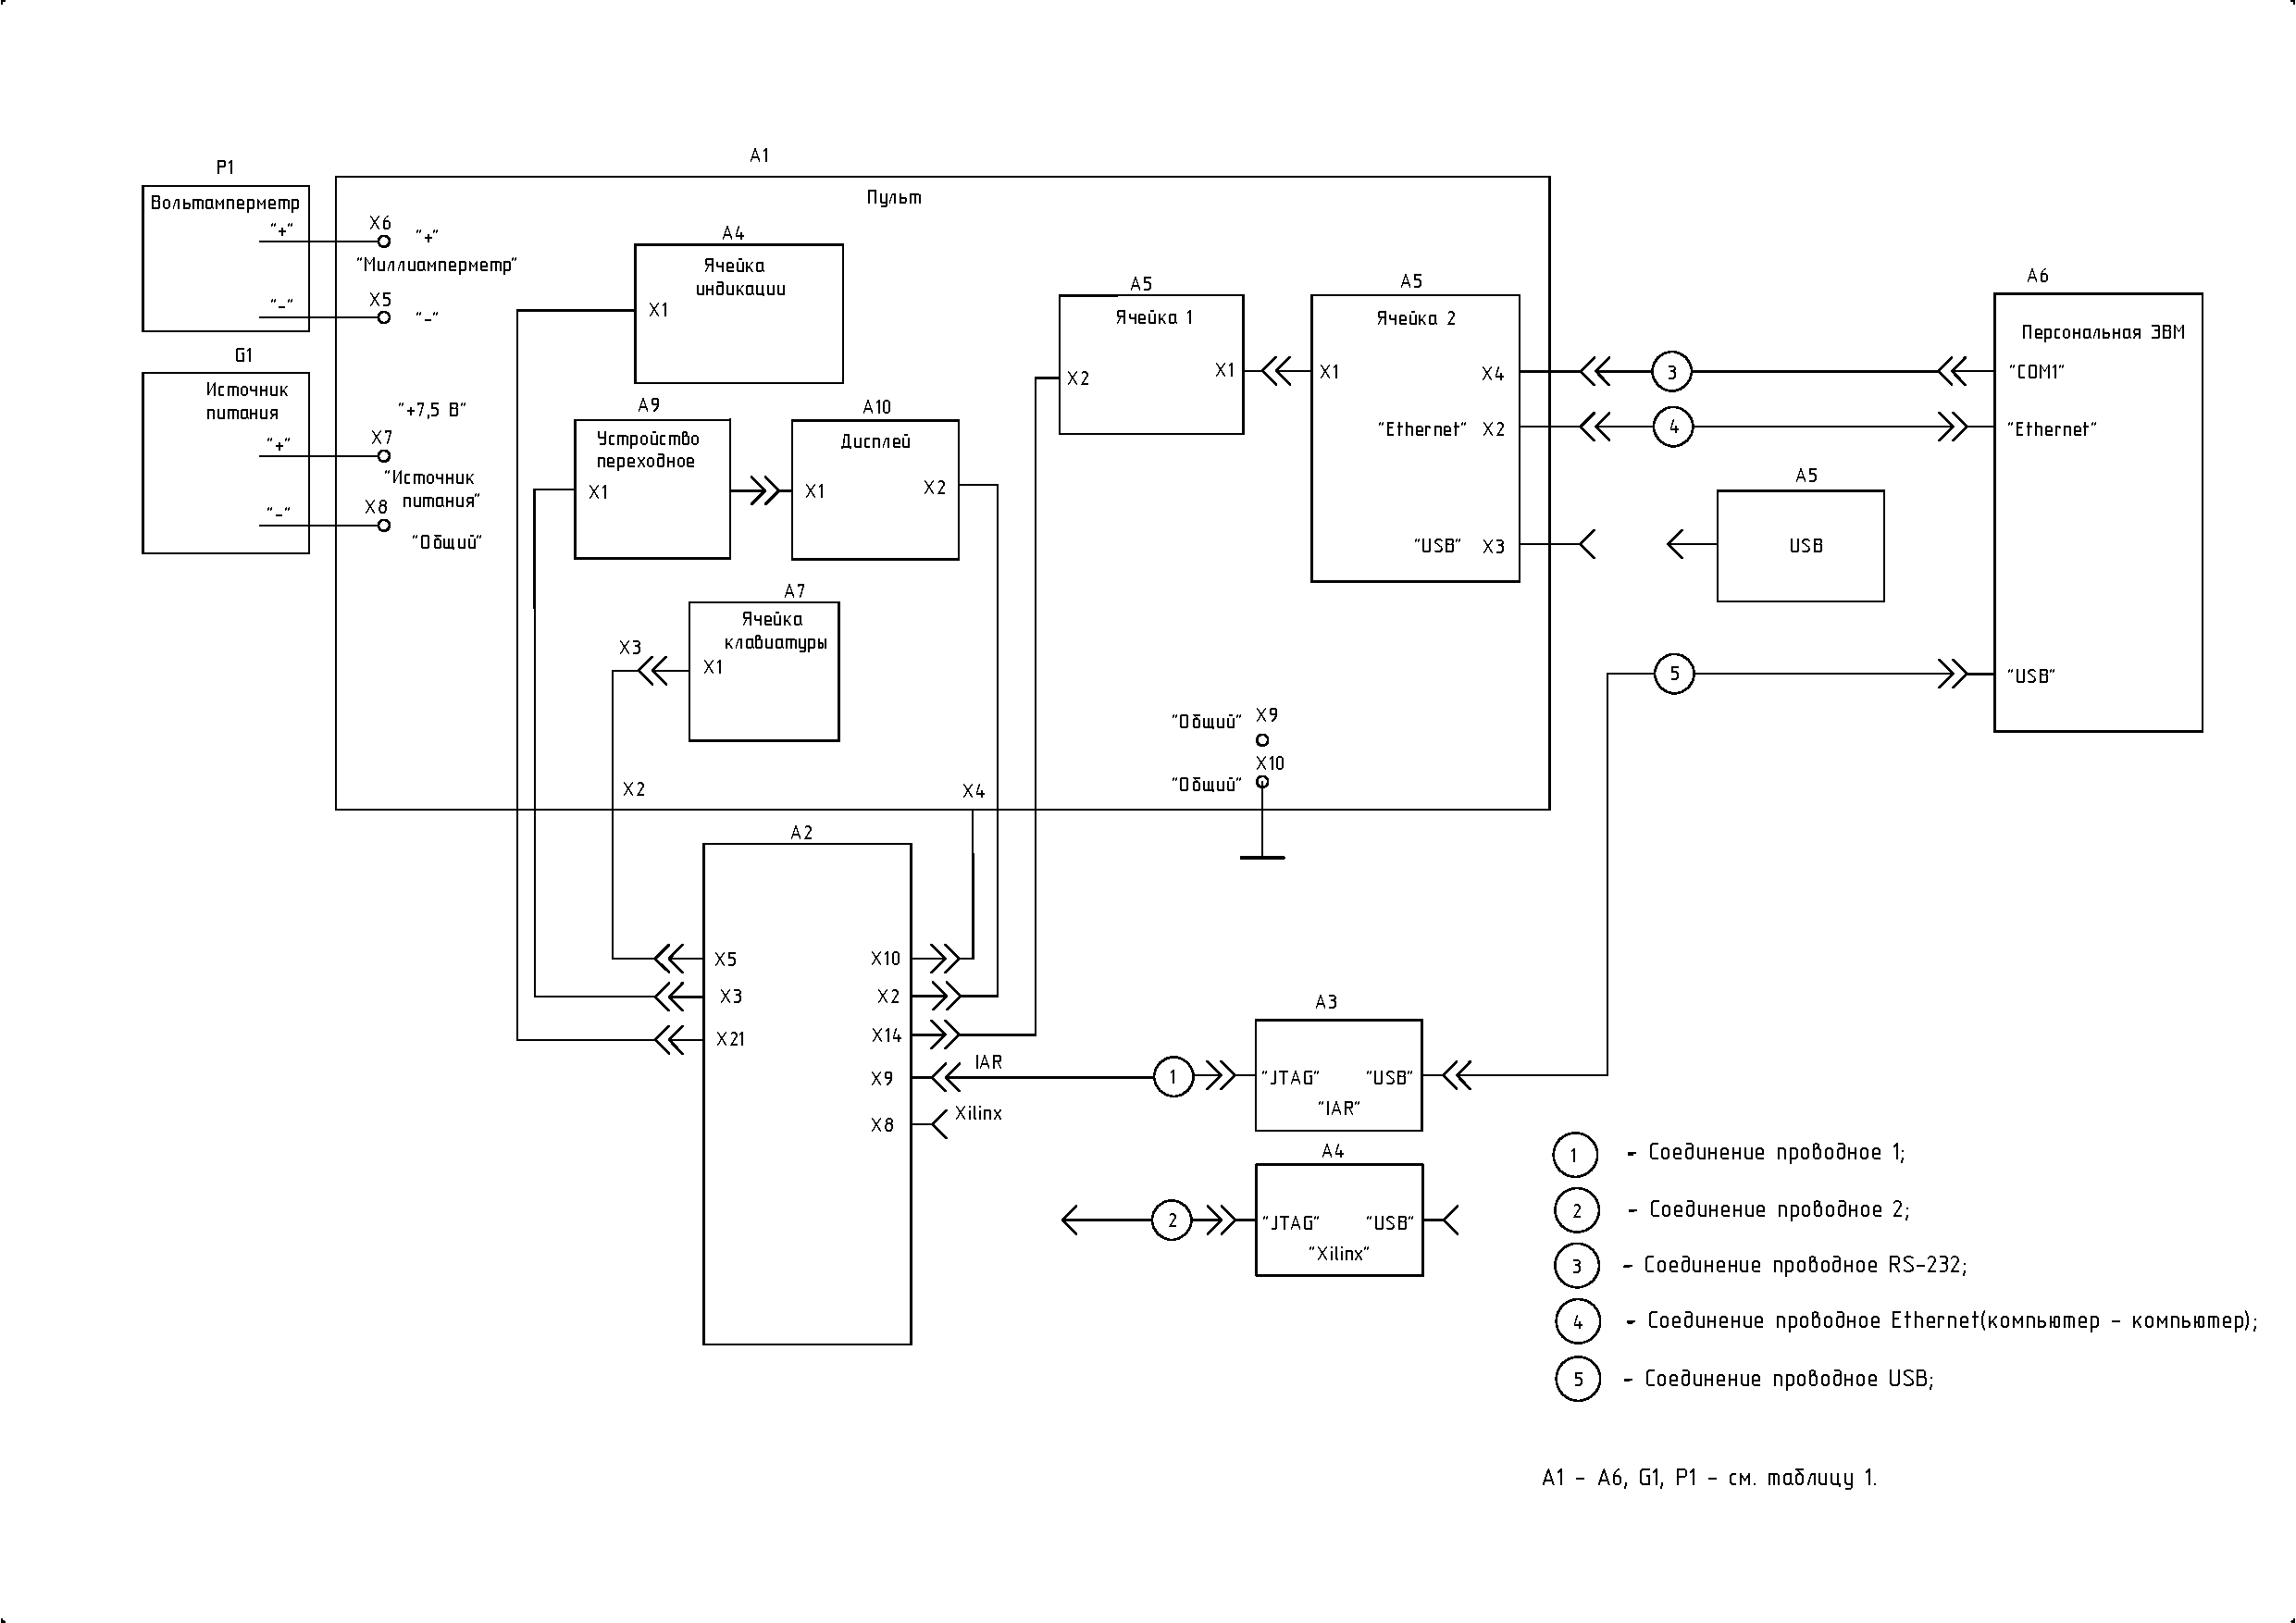
\includegraphics[ scale=1, angle=-90]{./about/A3_example}}% Волшебные чиселки. Их лучше не трогать, а то картинки расползутся и подпись к рисунку уползёт
  \end{picture}%

  \captionsetup{width=170mm,
                margin={-50mm,-150mm}
                }%
  \caption{Схема электрическая подключения устройства} \label{a:p:SCH_all_units}
\end{figure}%

}%




\FormatSizeA{43}{%

\begin{figure}[H]%
\unitlength=1mm%
  \begin{picture}(0,235)(26,50)% Волшебные чиселки. Их лучше не трогать, а то картинки расползутся и подпись к рисунку уползёт
    \put(0,0){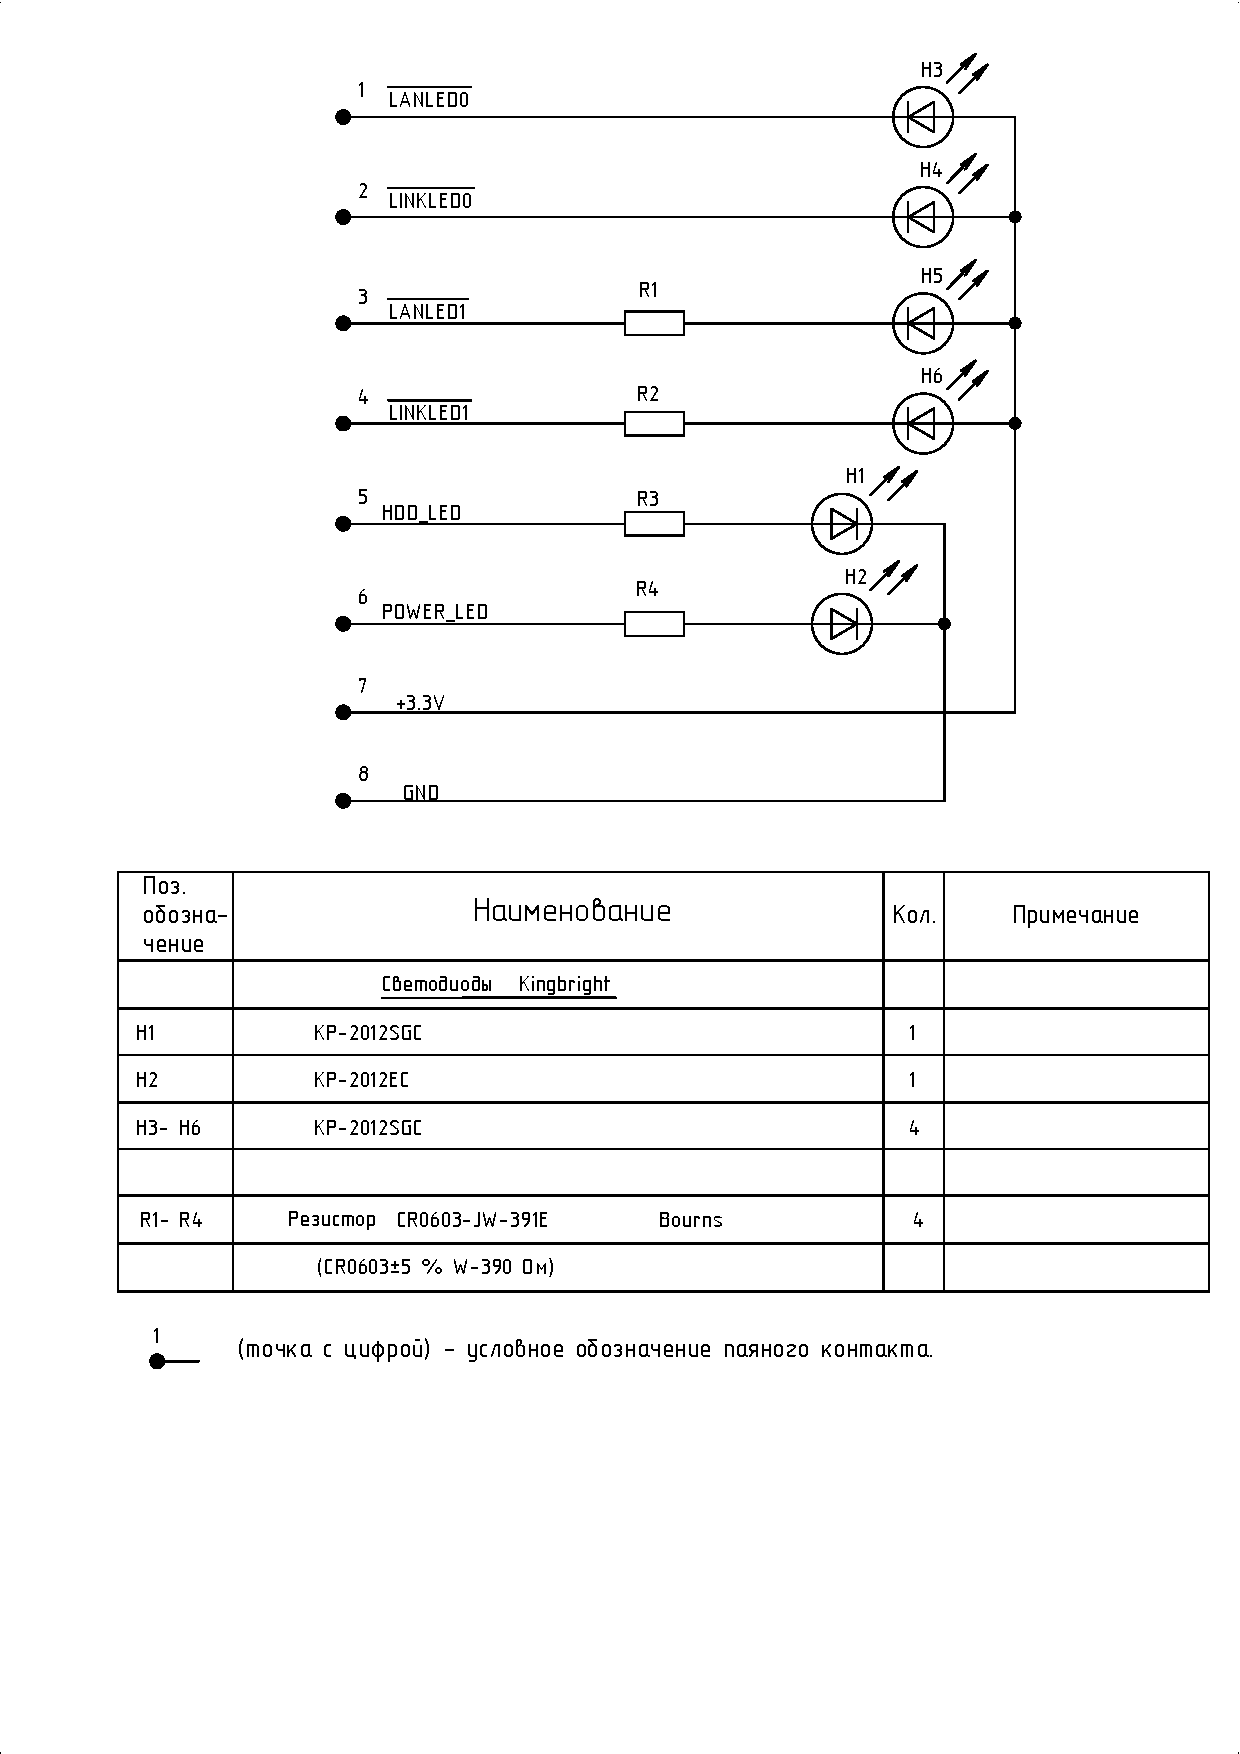
\includegraphics[scale = 1.004]{./about/A4_v_example}}% Волшебные чиселки. Их лучше не трогать, а то картинки расползутся и подпись к рисунку уползёт
  \end{picture}%
  \caption{Схема электрическая принципиальная ячейки индикации} \label{a:p:pult_main_part20}
\end{figure}%

}%







